\documentclass[12pt,a4paper,oneside,openright,titlepage]{report}
\usepackage[utf8]{inputenc}
\usepackage{amsmath}
\usepackage{amsfonts}
\usepackage{amssymb}
\usepackage {setspace}
\usepackage{graphicx}
%\usepackage{times}
\DeclareGraphicsExtensions{.png,.jpg}
\graphicspath{ {./images/} }
\usepackage {hyperref}
\usepackage[numbers,sort&compress]{natbib}
\usepackage{pdfpages}
\author{Mohan S Nayaka}
\title{Wave propagation Studies for Nanostructures}
\pagestyle{headings}
\begin{document}
\pagestyle{empty}
\includepdf[pages=-]{1_front_mohan.pdf}
\includepdf[pages=-]{2_bonafide_Mohan.pdf}
\includepdf[pages=-]{3_Declaration.pdf}
\includepdf[pages=-]{4_CSIR_Center_for_Mathematical_Modeling_Mohan.pdf}
\pagestyle{headings}
%\maketitle
\tableofcontents
\listoffigures
\chapter* {Abstract}
This is a study of wave propagation studies in a few different scenarios. We study the axial wave propagation in:\\
\begin{itemize}
\item Carbon nanorods
\item Carbon nanorods in elastic medium
\item Double nanorod system in elastic medium
\end {itemize}

%\setstretch {1.5}
\chapter* {Acknowledgments}
%\chapter*{Acknowledgements}
I place on record and warmly acknowledge the continuous
encouragement, invaluable supervision timely suggestions and inspired
guidance offered by our guide Mr.V. Senthilkumar, Senior Scientist, CSIR
Fourth Paradigm Institute (CSIR-4PI), NAL Belur Campus, Bangalore and
Prof. Manojkumar T.K., (Associate Professor, Indian Institute of Information Technology and Management - Kerala (IIITM-K)) in bringing this Project to a successful completion.

My sincere gratitude to Mr Shyam Chetty, Head, CSIR Fourth
Paradigm Institute (CSIR-4PI), Dr T R Ramamohan, former Acting Head,
CSIR-4PI, and Prof. P Seshu, former Head, Belur Campus, Bangalore, for
providing me the opportunity to work in CSIR-4PI.

I would like to thank the SPARK Team that provided me this
opportunity to carry out my project in this intellectually stimulating environment.

I extend my gratitude to C-MMACS Scientists and staff members
who supported me and allowed to get in touch with emerging research developments.

I extend my gratefulness to one and all who are directly or indirectly
involved in the successful completion of this project work.


\chapter {Introduction}
\section {Nanomaterials and Nanostructures}
A nanostructure is defined as a material system or object, where
at least one of the dimensions lies below 100 nm. Nanostructures
can be classified into three different categories:
\begin{enumerate}
\item zero-dimensional (0D)
\item one-dimensional (1D)
\item two-dimensional (2D)
\end{enumerate}
0D nanostructures are materials in which all three dimensions are at the nanoscale. A good example of these materials are buckminster fullerenes  and quantum dots. 1D nanostructures are materials that have two physical dimensions in the nanometer range, while the third dimension can be large, such as in the carbon nanotube. 2D nanostructures, or thin films, only have one dimension in the nanometer range and are used readily in the processing of complimentary metal-oxide semiconductor transistors and micro-electro-mechanical systems (MEMS). Nanomaterials are the base material of many nanoscale objects. Recently various one-dimensional nanostructures have been realized. They include nanodots, nanorods, nanowires, nanobelts, nanotubes, nanobridges and nanonails, nanowalls, nanohelices, seamless nanorings. Among all the one-dimensional nanostructures, nanotubes, nanorods and nanowires are widely studied. This is because of the easy material formation and device applications.

Nanostructures have unique properties when compared to their individual atoms or
molecules or their bulk macroscopic properties. For example, bulk material such as
Copper wire, their intrinsic properties, say density or conductivity, are independent
of its size. That is, if a 1 m long Copper wire, when cut into few pieces, and for these pieces, if the density or conductivity is measured, one will find they are same as the original Copper wire. If the dividing process is done indefinitely, then the property invariance will still remain. However, if the division is made at the electron, proton or neutron levels, that is at the nanoscale levels, we can certainly expect significant change in the property of the nanostructures. The properties of the nanoscale material systems can get significantly affected by the following three phenomenon:
\begin{itemize}
\item \textit{Quantum Confinement}: The confinement of electrons in the nanoscale dimensions will result in the change in the energy and momentum of the nano material system, which in turn significantly alters its properties.
\item \textit{Quantum Coherence}: : This phenomenon relates to the phase relation of the wave function in nano material system, that is preserved in the nanomaterial system. The quantum coherence property is well maintained in atoms and molecules but not always in nanostructures due to inherent defects present in these structures.
This results in the change of properties in the nano scale and hence it is necessary
to consider both the quantum coherence and de-coherence effects while dealing
with nanostructures.
\item \textit{Surface Effects}: Vast majority of the atoms in a nanostructures are located either at the surfaces or interfaces. The properties of these surface atoms can be quite different than that of those, which are located in the interior.
\end{itemize}

The above factors significantly alter the properties of the nanostructures as compared to their bulk material. For a nanomaterial systems, both the crystalline state and surface/interface state is very important. These materials are often in metastable state. Their atomic configuration depends on the kinetic process in which they are fabricated or grown. Therefore, the properties of nanostructures can be adjusted or manipulated by changing its size, shape or the process by which it is made, which can often lead to some rich and surprising outcomes.

\section {Carbon Nanotubes}
Carbon is a remarkable element that has a unique structures which make it amenable
to combine with other elements and compounds to get a new compound. It is said
that carbon has the ability for form close to 10 million different compounds. It is
present in the food we eat, the clothes we wear, the cosmetics we use and also in
the fuel that drives our cars. Carbon exists in four different allotropes, namely the
amorphous, the graphite, the diamond and the fullerene. The Amorphous carbon
structure is visually a highly disordered structure. It is for this reason that it lacks
structural integrity . This carbon structure forms at the edges or is the residue of other
elemental compounds. The disorder of this structure allows it to have many available
bonds and is responsible for building more complex carbon based molecules.

There are many definitions to nanotubes. The simplest definition of nanotube is that
it is a nanometer scale structure that resembles a tube. There are both organic and
inorganic nanotubes. Organic nanotubes are the carbon nanotubes or CNT. With
respect to Carbon NanoTube (CNT), a nanotube can be defined as \emph{a long cylindrical carbon structure
consisting of hexagonal graphite molecules attached at the edges}. Some nanotubes
have a single cylinder while others have two or more concentric cylinders. Nanotubes
have several characteristics, namely wall thickness, number of concentric cylinders,
cylinder radius, and cylinder length. Some nanotubes have a property called chirality,
an expression of longitudinal twisting.

\subsection {Types and structures}
Carbon nanotubes are basically sheets of graphite rolled up into a tube as shown in this figure. Hence, the hexagonal two dimensional lattice of graphite is mapped on a one-dimensional cylinder of radius R with various helicities characterized by the rolling vectors (n,m).\cite{types_taner} Nanotubes form different types, which can be described by the chiral vector $(n, m)$, where $n\text{ and }m$ are integers of the vector equation $R = n a_1 + m a_2$. The chiral vector is determined by the diagram at the left. Imagine that the nanotube is unraveled into a planar sheet. Draw two lines (the blue lines) along the tube axis where the separation takes place. In other words, if you cut along the two blue lines and then match their ends together in a cylinder, you get the nanotube that you started with. Now, find any point on one of the blue lines that intersects one of the carbon atoms (point A). Next, draw the Armchair line (the thin yellow line), which travels across each hexagon, separating them into two equal halves. Now that you have the armchair line drawn, find a point along the other tube axis that intersects a carbon atom nearest to the Armchair line (point B). Now connect A and B with our chiral vector, $R$ (red arrow). The wrapping angle $\phi$; (not shown) is formed between $R$ and the Armchair line. If $R$ lies along the Armchair line ($\phi=0^\circ$), then it is called an "\textit{Armchair}" nanotube. If $\phi=30^\circ$, then the tube is of the "\textit{zigzag}" type. Otherwise, if $\phi \ll 30^\circ$ then it is a "\textit{chiral}" tube. The vector $a_1$ lies along the "\textit{zigzag}" line. The other vector $a_2$ has a different magnitude than $a_1$, but its direction is a reflection of $a_1$ over the Armchair line. When added together, they equal the chiral vector $R$.
The values of $n\text{ and }m$ determine the chirality, or "twist" of the nanotube. The chirality in turn affects the conductance of the nanotube, it's density, it's lattice structure, and other properties. A SWNT is considered metallic if the value $n - m$ is divisible by three. Otherwise, the nanotube is semiconducting. Consequently, when tubes are formed with random values of n and m, we would expect that two-thirds of nanotubes would be semi-conducting, while the other third would be metallic, which happens to be the case.\cite{eqstruct}
Given the chiral vector (n,m), the diameter of a carbon nanotube can be determined using the relationship\\
\[d = (n^2 + m^2 + nm)^{1/2} \times 0.0783 nm\]
\begin{figure}
\centering
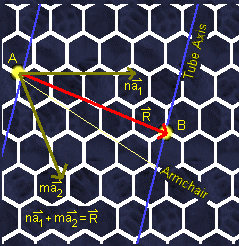
\includegraphics[scale=1]{typesNT.png}
\caption{Illustration of rolling vectors (n,m)}
\label{typesNT}
\end{figure}
\begin{figure}
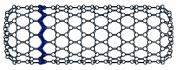
\includegraphics[scale=1]{n0tube.jpg}
\caption{(n,0) zigzag nanotube }
\label{n0tube}
\end{figure}
\begin{figure}
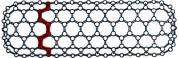
\includegraphics[scale=1]{nntube.jpg}
\caption{(n,n) armchair nanotube}
\label{nntube}
\end{figure}
\begin{figure}
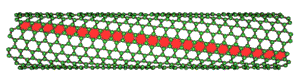
\includegraphics[scale=1]{nmtube.png}
\caption{(n,m) chiral nanotube}
\label{nmtube}
\end{figure}
\subsection {Why study Carbon nanotubes?}
Carbon nanotubes are molecular-scale tubes of graphitic carbon with outstanding properties. They are among the stiffest and strongest fibres known, and have remarkable electronic properties and many other unique characteristics. For these reasons they have attracted huge academic and industrial interest, with thousands of papers on nanotubes being published every year. Commercial applications have been rather slow to develop, however, primarily because of the high production costs of the best quality nanotubes.

The current huge interest in carbon nanotubes is a direct consequence of the synthesis of buckminsterfullerene, $C_{60}$, and other fullerenes, in 1985. The discovery that carbon could form stable, ordered structures other than graphite and diamond stimulated researchers worldwide to search for other new forms of carbon. The search was given new impetus when it was shown in 1990 that $C_{60}$ could be produced in a simple arc-evaporation apparatus readily available in all laboratories. It was using such an evaporator that the Japanese scientist Sumio Iijima discovered fullerene-related carbon nanotubes in 1991\cite{iijima1991helical}. The tubes contained at least two layers, often many more, and ranged in outer diameter from about 3 nm to 30 nm. They were invariably closed at both ends.

The strength of the $\mathrm{sp^2}$ carbon-carbon bonds gives carbon nanotubes amazing mechanical properties. The stiffness of a material is measured in terms of its Young's modulus, the rate of change of stress with applied strain. The Young's modulus of the best nanotubes can be as high as 1000 GPa which is approximately 5x higher than steel. The tensile strength, or breaking strain of nanotubes can be up to 63 GPa, around 50x higher than steel. These properties, coupled with the lightness of carbon nanotubes, gives them great potential in applications such as aerospace. It has even been suggested that nanotubes could be used in the “space elevator”, an Earth-to-space cable first proposed by Arthur C. Clarke. The electronic properties of carbon nanotubes are also extraordinary. Especially notable is the fact that nanotubes can be metallic or semiconducting depending on their structure. Thus, some nanotubes have conductivities higher than that of copper, while others behave more like silicon. There is great interest in the possibility of constructing nanoscale electronic devices from nanotubes, and some progress is being made in this area. However, in order to construct a useful device we would need to arrange many thousands of nanotubes in a defined pattern, and we do not yet have the degree of control necessary to achieve this. There are several areas of technology where carbon nanotubes are already being used. These include flat-panel displays, scanning probe microscopes and sensing devices. The unique properties of carbon nanotubes will undoubtedly lead to many more applications.\cite{importance}
\subsection {Why study wave propagation in CNTs?}
Increasing emphasis of miniature devices have made the scientists to look for newer
and novel materials which can be handled at the atomistic scales. In this regard,
Nanoscale materials and structures with nano thicknesses have attracted consider-
able interest from the scientific community in the fields of microelectronics and
nanotechnology. More and more nanostructures, e.g. ultra-thin films, nanowires
and nanotubes, have been fabricated and served as the basic building blocks for
nano-electro-mechanical-systems (NEMS). For long-term stability and reliability of
various devices at nanoscale, researchers should possess a deep understanding and
knowledge of mechanical properties of nano-materials and -structures, especially the
time dependent or dynamic properties.

Nanostructures such as CNTs can propagate waves of the order of terahertz (THz). As dimensions of the material become smaller, however, their resistance to deformation is increasingly determined by internal or external discontinuities (such as surfaces, grain boundary, strain
gradient, and dislocation). Although many sophisticated approaches for predicting
the mechanical properties of nanomaterials have been reported, few addressed the
challenges posed by interior nanostructures such as the surfaces, interfaces, struc-
tural discontinuities and deformation gradient of the nanomaterials under extreme
loading conditions. The use of atomistic simulation may be a potential solution in
the long run. However, it is well known that the capability of this approach is much
limited by its need of prohibitive computing time and an astronomical amount of data
generated in the calculations. Wave propagation analysis using continuum models,
especially using non-local elasticity models can used to address the above problems.

Wave propagation studies mainly include the estimation of wavenumber and wave
speeds such as phase and group speeds. The concept of group velocity may be useful
in understanding the dynamics of carbon nanotubes, since it is related to the energy
transportation of wave propagation. It is useful to study the
wave propagation in nanostructures, so as to examine the effect of length scales on
the wave dispersion from the viewpoint of group velocity or energy transportation. To
describe the effect of microstructures of a nanostructures on its mechanical properties,
it is assumed that the model of the nanostructure is made of a kind of non-local elastic
material, where the stress state at a given reference location depends not only on the
strain of this location but also on the higher order gradient of strain, so as to take
the influence of the microstructures into account. It is reported that both local elastic
models (where effects of nano scale is not considered) and non-local elastic models
(where the effect of scale is considered) can offer the correct prediction when the
wavenumber is lower. However, the results of the elastic model remarkably deviate
from those given by the non-local elastic model with an increase in the wavenumber.
As a result, the microstructures play an important role in the dispersion of waves in
nanoscale structures. Since terahertz physics of nanoscale materials and devices are
the main concerns in wave characteristics of CNTs, the small-scale effect must be
of significance in achieving accurate dispersion relations as the wavelength in the
frequency domain is in the order of nanometers.\cite{gopalakrishnan2013wave}

\chapter {Continuum Mechanics}
\section {Fundamental Concepts}
Continuum mechanics is a branch of mechanics that deals with the analysis of the kinematics and the mechanical behaviour of materials modelled as a continuous mass rather than as discrete particles. The French mathematician Augustin-Louis Cauchy was the first to formulate such models in the 19th century, but research in the area continues today.

Modelling an object as a continuum assumes that the substance of the object completely fills the space it occupies. Modelling objects in this way ignores the fact that matter is made of atoms, and so is not continuous; however, on length scales much greater than that of inter-atomic distances, such models are highly accurate. Fundamental physical laws such as the conservation of mass, the conservation of momentum, and the conservation of energy may be applied to such models to derive differential equations describing the behaviour of such objects, and some information about the particular material studied is added through constitutive relations.

Continuum mechanics deals with physical properties of solids and fluids which are independent of any particular coordinate system in which they are observed. These physical properties are then represented by tensors, which are mathematical objects that have the required property of being independent of coordinate system. These tensors can be expressed in coordinate systems for computational convenience.

Materials, such as solids, liquids and gases, are composed of molecules separated by ``empty'' space. On a microscopic scale, materials have cracks and discontinuities. However, certain physical phenomena can be modeled assuming the materials exist as a continuum, meaning the matter in the body is continuously distributed and fills the entire region of space it occupies. A continuum is a body that can be continually sub-divided into infinitesimal elements with properties being those of the bulk material.

The validity of the continuum assumption may be verified by a theoretical analysis, in which either some clear periodicity is identified or statistical homogeneity and ergodicity of the microstructure exists. More specifically, the continuum hypothesis/assumption hinges on the concepts of a representative volume element (RVE) (sometimes called "representative elementary volume") and separation of scales based on the Hill–Mandel condition. This condition provides a link between an experimentalist's and a theoretician's viewpoint on constitutive equations (linear and nonlinear elastic/inelastic or coupled fields) as well as a way of spatial and statistical averaging of the microstructure.\cite{wiki:cm}

Continuum mechanics models begin by assigning a region in three-dimensional Euclidean space to the material body $\mathcal{B}$ being modeled. The points within this region are called particles or material points. Different configurations or states of the body correspond to different regions in Euclidean space. The region corresponding to the body's configuration at time $t$ is labeled $\kappa_t(\mathcal{B})$.
\begin{figure}
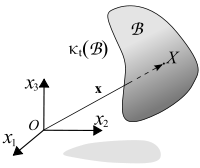
\includegraphics[scale=0.75]{Continuum_body}
\caption{Configuration of a continuum body}
\label{continuumbody}
\end{figure}

A particular particle within the body in a particular configuration is characterized by a position vector\\
\[\mathbf{x} = \sum_{i=1}^3x_i \mathbf{e}_i\]
where $\mathbf{e}_i$ are the coordinate vectors in some frame of reference chosen for the problem (see Fig.\ref{continuumbody}. This vector can be expressed as a function of the particle position $\mathbf{X}$ in some reference configuration, for example the configuration at the initial time, so that\\
\[\mathbf{x}=\kappa_t(\mathbf{X})\]\\
This function needs to have various properties so that the model makes physical sense. $\kappa_t(\cdot)$ needs to be:\\
\begin{itemize}
\item continuous in time, so that the body changes in a way which is realistic,
\item globally invertible at all times, so that the body cannot intersect itself,
\item orientation-preserving, as transformations which produce mirror reflections are not possible in nature.
\end{itemize}
For the mathematical formulation of the model, $\kappa_t(\cdot)$ is also assumed to be twice continuously differentiable, so that differential equations describing the motion may be formulated.

\section {Non-local mechanics}
This theory assumes that the stress state at a reference point $\mathbf{x}$ in
the body is regarded to be dependent not only on the strain state at
$\mathbf{x}$ but also on the strain states at all other points $x$ of the body. The
most general form of the constitutive relation in the nonlocal
elasticity type representation involves an integral over the entire
region of interest. The integral contains a nonlocal kernel function,
which describes the relative influences of the strains at various
locations on the stress at a given location. The constitutive
equations of linear, homogeneous, isotropic, nonlocal elastic solid
with zero body forces are given by\\
\begin{equation}
\sigma_{ij,j}=0
\end{equation}
\begin{equation}
\sigma_{ij}(\mathbf{x})=\int_V \alpha(|\mathbf{x-x'}|,\xi)C_{ijkl}\varepsilon_{kl}(\mathbf{x'})dV(\mathbf{x'}),\qquad \forall x \in V \label{eqNL}
\end{equation}
\begin{equation}
\varepsilon_{ij}=\frac{1}{2}(u_{i,j}+u_{j,i})
\end{equation}
where $C_{ijkl}$ is the elastic modulus tensor of classical isotropic
elasticity, $\sigma_{ij}$ and $\varepsilon_{ij}$ are stress and strain tensors, respectively,
and $u_i$ is the displacement vector. $\alpha = \alpha(|\mathbf{x-x'}|,\xi)$ is the nonlocal
modulus or attenuation function incorporating the nonlocal effects
into the constitutive equations. This nonlocal modulus is found by
matching the curves of plane waves with those due to atomic lattice
dynamics. Various different forms of $\alpha(|\mathbf{x-x'}|)$ have been reported in \cite{eringen1976nonlocal} .$|\mathbf{x-x'}|$ is the Euclidean distance, and $\xi = e_0 a/l$\cite{peddieson2003application} where a is an internal characteristic length, e.g., length of C–C bond
(0.142 nm) in CNT, granular distance etc., and $l$ is an external
characteristic length e.g., wavelength ($\lambda$) , crack length, size of the
sample etc. $e_0$ is a nonlocal scaling parameter, which has been
assumed as a constant appropriate to each material in published
literature and V is the region occupied by the body. Choice of the
value of parameter $e_0a$  (in dimension of length) is crucial to ensure
the validity of nonlocal models. This parameter was determined by
matching the dispersion curves based on the atomic models\cite{eringen1983differential}. For
a specific material, the corresponding nonlocal parameter can be
estimated by fitting the results of atomic lattice dynamics or
experiment.

The generally used kernel function $\alpha(|\mathbf{x-x'}|,\xi)$ used in \ref{eqNL} is given in \cite{eringen1972linear}:\\
\begin{equation}
\alpha(|\mathbf{x-x'}|,\xi) = \dfrac{1}{2 \pi \xi^2 l^2} K_0\left(\frac{\bf{x.x}}{\xi l}\right)
\end{equation}
where $K_0$ is is the modified Bessel function.
For two-dimensional nonlocal elasticity, there exists a differential form for the stress–strain relation (from Eq. \eqref{eqNL})\cite{eringen1972linear,eringen1976nonlocal,eringen1983differential,eringen1972nonlocal}\\
\begin{equation}
\left(1-\xi^2 l^2 \nabla^2\right)\sigma_{ij} = C_{ikjl}\varepsilon_{kl} \label{NLconsteqn}
\end{equation}
where the operator $\nabla^2$ is the Laplacian operator. Notice that in the
nonlocal elasticity, the effect of small-length scale is considered by
incorporating the internal parameter length into the constitutive
equation. One may also see that when the internal characteristic
length $a$ is neglected, i.e., the particles of a medium are considered
to be continuously distributed, then $\xi =0$ and \eqref{NLconsteqn} reduces to the
constitutive equation of classical elasticity. When the internal
characteristic length is negligible compared to external characteristic length, $\xi$ approaches zero and hence nonlocal elasticity theory reduces to classical elasticity theory. While the internal characteristic length is reasonably close to external characteristic length, $\xi$ approaches to unity and thus the nonlocal elasticity
theory reduces to atomic lattice dynamics. For nanostructures, the
internal and external lengths are of the same order, and one has to
use the nonlocal theory for analysis.
\subsection{Discussion on nonlocal small scale coefficient}
The identification of the small scaling parameter $e_0$ in the
nonlocal theory has not been fully understood. Wang and Hu \cite{wang2005flexural},
who adopted the second order strain gradient constitutive relation,
proposed $e_0 = 0.288$ for the flexural wave propagation study in a
single-walled carbon nanotube (SWCNT) through the use of
nonlocal Timoshenko beam model and molecular dynamic simulations (MDSs).Eringen \cite{eringen1983differential} himself proposed $e_0$ as 0.39 based on the
matching of the dispersion curves via nonlocal theory for plane wave and Born-K\'arm\'an model of lattice dynamics at the end of
the Brillouin zone, $k \times a = \pi$ where $a$ is the distance between atoms
and $k$ is the wave number in the phonon analysis. On the other
hand, Eringen \cite{eringen1972linear}proposed $e_0 =0.31$ in his study on the comparison of the Rayleigh surface wave via nonlocal continuum mechanics
and lattice dynamics. Zhang et al.\cite{zhang2005free} estimated $e_0=0.82$ from the buckling analysis of SWCNT via Donnell shell theory and molecular
mechanics simulations. Zhang et al.\cite{zhang2006atomistic} performed analysis of
elastic interactions between Stone–Wales and divacancy defects on
carbon graphene sheet. They concluded that the displacement field
around defects obtained from the nonlocal continuum model and
MDSs can match very well if $e_0$ is chosen to be $8.79$  The varied
values of $e_0$ prompted Wang \cite{wang2005wave} to state that the adopted value of
the scaling parameter $e_0$ depends on the crystal structure in lattice
dynamics and the nature of physics under investigation. He also
estimated that the scale coefficient $e_0 < 2.0$ nm for a SWCNT if the
measured wave propagation frequency value is assessed to be
greater than 10 THz. Although $e_0$ is a key parameter in the nonlocal
elasticity theory, there is hitherto no rigorous study being made on
estimating the scaling parameter $e_0$ for various physical problems.
Hu et al.\cite{hu2008nonlocal} estimated the value of parameter $e_0$ is estimated
based on the MD result to predict the dispersion of transverse wave
in CNTs through using the nonlocal shell models. The results of
their study indicate that the nonlocal elastic cylindrical shell model
is able to offer a better prediction for transverse and torsional wave
dispersion in CNTs than the local elastic shell model when the
wavenumber is large enough. They also show that the nonlocal
shell models are required when the wavelengths are approximately
less than $2.36 \times 10^{-9} \text{ and } 0.95 \times  10^{-9}$m for transverse wave in armchair (15,15) SWCNT and torsional wave in armchair (10,10)
SWCNT, respectively. Following Wang \cite{wang2005wave}, the nonlocal parameter $e_0a$ should be less than 2.0 nm, so that here in the simulation procedure we choose
$e_0a = 0.0, 0.5\text{ and }1.0 $ nm, respectively.


\chapter {Wave Propagation}
\section {Fundamental Concepts}
Wave propagation is any of the ways in which waves travel.
With respect to the direction of the oscillation relative to the propagation direction, we can distinguish between longitudinal wave and transverse waves.
For electromagnetic waves, propagation may occur in a vacuum as well as in a material medium. Other wave types cannot propagate through a vacuum and need a transmission medium to exist.\cite{wiki:wp}

\subsection*{Wavenumber and Wave Frequency \cite{mitocwwp}}
If the range of the spatial corrdinate x is $(-\infty,\infty)$,and all coefficients are independent of $x,t$,  then the first task is to examine the physics
of sinusoidal wave train of the form:\\
\[V(x,t) = |A|cos(kx - \omega t - \phi_A)=\mathfrak{R}(A e^{ikx-i\omega t})\]
where $A = |A| e^{i \phi_A}$ is a complex number with magnitude $|A|\text{ and phase angle} \phi_A$ After
examining the physical meaning of this special type of waves, it is possible to use the
principle of superposition to construct more general solutions. It is customary to omit
the symbol $\mathfrak{R} = $ ``the real part of''  for the sake of brevity, i.e.,\\
\[V(x,t) = Ae^{ikx-i\omega t}\]
\emph{Definition}: We shall call:\\
\begin{center}
\framebox{$\theta(x,t) = kx - \omega t$}\\
\end{center}
the \emph{wave phase}. Clearly the trigonometric function is periodic in phase with the period $2 \pi$. In the $x,t$ plane, $V$ has a constant value along a line of contant phase. In particular, $\theta = 2n \pi$ correspond to the wave crests where $V = |A|$ is the greatest.
On the other hand, $\theta = (2n+1) \pi (n=1,2,3,\ldots$ correspond to the wave troughs where $V = -|A|$ is the smallest. $|A|$ is half of the separation between adjacent crests
and troughs and is called the \emph{wave amplitude}; we also call A the complex amplitude. Clearly $\frac{\partial \theta}{\partial x}$ represents the number of phase lines per unit distance, i.e., the density of
phase lines, at a given instant; it is called the \emph{wave number}.\\
\begin{center}
\framebox{$\text{wave number} = k = \frac{\partial \theta}{\partial x}$}
\end{center}
On the other hand $-\frac{\partial \theta}{\partial t}$ represensts the number of phase lines passing across a fixed x per unit time; it is called the \emph{wave frequency}.\\
\begin{center}
\framebox{$\text{wave frequency} = \omega = \frac{\partial \theta}{\partial t}$}
\end{center}
To stay with a particular line of contant phase, say a crest, one must have\\
\[d\theta = k dx -\omega dt = 0\]
namely one must move at the \emph{phase velocity},\\
\begin{center}
\framebox{$c = \left.\frac{dx}{dt}\right|_{\theta=constant} = \frac{\omega}{k}$}
\end{center}
In general a sinusoidal wave whose
phase velocity depends on the wavelength, i.e.,$\omega$ is a nonlinear function of $k$, is called a \emph{dispersive wave}. We define the \emph{group velocity} as:
\begin{center}
\framebox{$\text{group velocity} = c_g = \frac{d\omega}{dt}$}
\end{center}

\chapter {Studies conducted}
\section{Terahertz Wave Propagation in uniform nanorods}
\subsection*{Introduction}
The dynamic testing of materials and components often involves predicting the propagation of stress waves in slender rods. The present work deals with the analysis of the wave propagation characteristics of nanorods. The nonlocal elasticity theory and also the lateral inertia are incorporated into classical/local rod model to capture unique features of the nanorods under the umbrella of continuum mechanics theory.
The strong effect of the nonlocal scale has been obtained which leads to substantially different wave behaviors of nanorods from those of macroscopic rods. Nonlocal rod/bar model is developed for nanorods including the lateral inertia effects. The analysis shows that the wave characteristics are highly overestimated by the classical rod model, which ignores the effect of small-length scale. The wave propagation properties of the nanorod obtained from the present formulations are compared with the continuum rod model, nonlocal second and fourth order strain gradient models, Born-Karman model and the nonlocal
stress gradient model. It has also been shown that, the unstable second order strain gradient model can be replaced by considering the inertia gradient terms in the formulations. The effects of both the nonlocal scale and the diameter of the nanorod on spectrum curves are studied.

\subsection{Nonlocal governing partial differential equation for nanorods}
Figure \ref{nanorod} schematically describes a nanorod under discussion and
serves to introduce the axial coordinate x, lateral coordinate y, the
axial displacement $u = u(x,t)$the Young’s modulus $E$, the density $\rho$ the Poisson’s ratio $\nu$ and cross-sectional area $A$ . The displacement
field (X-direction), strain, strain rate and particle velocity associated with the displacement field in X-direction for this nanorod
are given by\\
\begin{equation}
u=u(x,t)
\end{equation}
\begin{equation}
\varepsilon_{xx}=\frac{\partial u}{\partial x}
\end{equation}
\begin{equation}
\dot{\varepsilon_{xx}}=\frac{\partial u}{\partial t} = \frac{\partial^2 u}{\partial x \partial t}
\end{equation}
\begin{equation}
V = \dot{u} = \frac{\partial u}{\partial t}
\end{equation}
\begin{figure}[b]
\centering
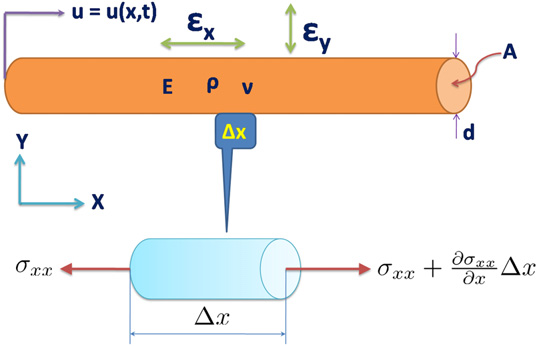
\includegraphics[scale=0.3]{nanorod}
\caption{A nanorod, showing Young’s modulus $E$, density $\rho$, Poisson’s ratio $\nu$, diameter $d$, cross-sectional area $A$, longitudinal displacement $u=u(x,t)$, strain along X-direction $\varepsilon_x$ and strains along Y-direction $\varepsilon_y$}
\label{nanorod}
\end{figure}
Due to Poisson’s ratio $\nu$, there are displacement fields $\nu$ and $w$ in
Y- and Z-directions, respectively. For example the strain and the
derivative of the displacement with time in the Y-direction are,
respectively,\\
\begin{equation}
\varepsilon_{yy}=-\nu \varepsilon_{xx}
\end{equation}
\begin{equation}
\dot{\nu}=-\nu y\dot{\varepsilon_{xx}}
\end{equation}
The kinetic energy of the infinitesimal length $\delta$ of the rod (from \ref{nanorod}) is:\\
\begin{equation}
\Delta \Pi^e = \frac{1}{2} \rho A \Delta x (V^2+\nu^2 \xi^2 \dot{\varepsilon}^2_{xx})
\end{equation}
where $\rho$ is the density, $A$ is the cross-sectional area and $\xi$ is the
radius of gyration of the solid circular cross-section. Here, an
effective density is used to incorporate the effect of lateral inertia in
a one-dimensional nonlocal wave equation. An effective density $\rho_{eff}$ is now introduced such that the kinetic energy of the element $\Delta x$ is $\Delta \Pi^e_{eff}$, where\\
\begin{equation}
\Delta \Pi^e_{eff} =\frac{1}{2} \rho_{eff} A \Delta x V^2
\end{equation}
Using Newton’s second law, the net longitudinal force acting on the
element $\Delta x$ (see \ref{nanorod}) is:\\
\begin{equation}
\Delta \sigma_{xx} \times A = \rho_{eff} A \frac{\partial^2 u}{\partial t^2} \times x
\label{rhoeff}
\end{equation}
In the limiting case as $\Delta x \rightarrow 0$, equation \ref{rhoeff} becomes:\\
\begin{equation}
\frac{\partial \sigma_{xx}}{\partial x} = \rho_{eff} \frac{\partial^2 u}{\partial t^2}
\label{limcasesigma}
\end{equation}
To find the relationship between $\rho_{eff}$ and $\rho$, a functional $\cup_e$ is defined as the kinetic energy error when using the effective density, i.e.,\\
\begin{equation}
\bigcup_e = \iint [\Delta \Pi^e - \Delta \Pi^e_{eff} ] dx dt = 
\iint \left[ \dfrac{1}{2} \rho A (V^2 + \nu^2 \xi^2 \dot{\varepsilon}^2_{xx}) - 
\left( \dfrac{1}{2} \rho_{eff} A V^2 \right) \right] dx dt
\label{functionaldef}
\end{equation}
substituting for strain rate and particle velocity in \eqref{functionaldef} the
minimization of $\cup_e$ requires minimization of the following functional:\\
\begin{equation}
\bigcap_e = \iint \left\lbrace (\rho - \rho_{eff}) \left[\dfrac{\partial u}{\partial t}\right]^2 + \rho \nu^2 \xi^2 \left[ \dfrac{\partial^2 u}{\partial x \partial t} \right]^2 \right\rbrace dx dt
\end{equation}
The integrand of the functional $\cap_e$ is\\
\begin{equation}
f\left(\dfrac{\partial u}{\partial t},\dfrac{\partial^2 u}{\partial x \partial t}\right) = (\rho - \rho_{eff}) \left[\dfrac{\partial u}{\partial t}\right]^2 + \rho \nu^2 \xi^2 \left[ \dfrac{\partial^2 u}{\partial x \partial t}\right]^2
\label{func2}
\end{equation}
In order to minimize $\cap_e$ in \eqref{func2}, the integrand must satisfy the following equation:\\
\begin{equation}
\dfrac{\partial^2}{\partial x \partial t} 
\left[
 \dfrac{\partial f \left(\frac{\partial u}{\partial t},\frac{\partial^2 u}{\partial x \partial t}  \right)}{\partial \frac{\partial^2 u}{\partial x \partial t}}  
\right] 
- 
\dfrac{\partial}{\partial t}
\left[ 
\dfrac{\partial f \left(\frac{\partial u}{\partial t},\frac{\partial^2 u}{\partial x \partial t}  \right)}{\partial \frac{\partial u}{\partial t}}  
\right] = 0
\label{func3}
\end{equation}
Therefore, \eqref{func3} is identical to the following partial differential equation:\\
\begin{equation}
\rho_{eff} \frac{\partial^2 u}{\partial t^2} = \rho \frac{\partial^2 u}{\partial t^2} - \rho \nu^2 \xi^2 \frac{\partial^4 u}{\partial x^2 \partial t^2}
\label{effectivedenseq}
\end{equation}
The equation \eqref{effectivedenseq} gives the relationship between the effective density
S
and the density that minimizes the effective density error,$\cup_e$ defined in \eqref{functionaldef},over the length of the nanorod and the time of
motion. Substituting this expression in Eq. \eqref{limcasesigma} gives\\
\begin{equation}
\dfrac{\partial \sigma_{xx}}{\sigma x} = \rho \dfrac{\partial^2 u}{\partial t^2} - \rho \nu^2 \xi^2 \dfrac{\partial^4 u}{\partial x^2 \partial t^2}
\end{equation}
The constitutive model employed here is that obtained from the
theory of nonlocal/nonclassical continuum mechanics. For thin
rods Eq. \eqref{NLconsteqn} can be written in the following one dimensional form\\
\begin{equation}
\sigma_{xx} = \alpha^2 \frac{\partial^2 \sigma_{xx}}{\partial x^2} = E \varepsilon_{xx} = E \frac{\partial u}{\partial x}
\label{onedimconst}
\end{equation}
where $E$ is the modulus of elasticity,$\sigma_{xx}$ and $\varepsilon_{xx}$ are the local stress
and strain components in the $x$ direction, respectively, and $\alpha=e_0 a$ nonlocal scaling parameter. Differentiating the Eq. \eqref{onedimconst}with respect to $x$ on both sides, gives\\
\begin{equation}
\frac{\sigma_{xx}}{\partial x} - \alpha^2 \frac{\partial^3 \sigma_{xx}}{\partial x^3} = E \frac{\sigma_{xx}}{\partial x} = E \frac{\partial^2 u}{\partial x^2}
\label{diffonedimconst}
\end{equation}
Substituting equation \eqref{effectivedenseq} in eq. \eqref{diffonedimconst} gives\\
\begin{equation}
E \dfrac{\partial^2 u}{\partial x^2} = \rho \dfrac{\partial^2 u}{\partial t^2} - \rho \nu^2 \xi^2 \dfrac{\partial^4 u}{\partial x^2 \partial t^2} - \alpha^2 \rho \dfrac{\partial^4 u}{\partial x^2 \partial t^2} + \alpha^2 \rho \nu^2 \xi^2 \dfrac{\partial^6 u}{\partial x^4 \partial t^2}
\label{nonlocalinertia}
\end{equation}
Equation \eqref{nonlocalinertia} is the consistent fundamental governing equation of
motion for nonlocal rod model including the effect of lateral inertia/
Poisson’s effect. When $\alpha = e_0 a = 0\text{ and } \nu = 0$ , it is reduced to the equation of local or classical rod model.

\subsection*{Terahertz wave characteristics of nanorods}
For analyzing the ultrasonic/terahertz wave dispersion char-
acteristics in nanorods, we assume that a harmonic type of wave
solution for the displacement field u(x,t) and it can be expressed in
complex form as \cite{gopalakrishnan2008spectral,doyle1989wave}\\
\begin{equation}
u(x,t) = \sum_{p=0}^{P-1} \sum_{q=0}^{Q-1}\hat{u}(x,\omega_q)e^{-(k_p x - \omega_q t)}
\label{harmonicsoln}
\end{equation}
where $P$ and $Q$ are the number of time sampling points and number
of spatial sampling points, respectively, and $j=\sqrt{-1}$. $\omega_q$ is the
circular frequency at the $q$th time sample. Similarly, $k_p$ is the axial
wavenumber at the $p$th spatial sample point. Substituting Eq. \eqref{harmonicsoln} into the governing partial differential equation (eq. \eqref{nonlocalinertia}) we get
the characteristic equation (dispersion relation). The dispersion
relation is solved for the wavenumbers or wave frequencies. The
wave frequency is a function of wavenumber $k$, the nonlocal scaling
parameter $\alpha = e_0 a$and the material properties ($E, \nu,\text{ and } \rho$ of the
nanorod. This shows a non-linear relation between wavenumber
and wave frequency i.e., the obtained axial waves in nanorod are
dispersive in nature. The present results are compared with
the results obtained from classical continuum model, second and fourth order strain gradient models, stress gradient model and Born-K\'arm\'an model. If $\alpha = 0$ and $\nu = 0$ the wavenumber is directly
proportional to wave frequency, which will give a non-dispersive
wave behaviour (explained in \cite{doyle1989wave})

\subsection*{Numerical results and discussion}
For the present analysis, a single-walled carbon nanotube is
assumed as a nanorod. The values of the radius, thickness, Young’s
modulus and density are assumed as 3.5 nm, 0.35 nm, 1.03 TPa,
and 2300 $\mathrm{kg/m^3}$ , respectively.
The present results are compared with the results obtained from
the following models:\\
\begin{itemize}
\item \textit{Classical/Local continuum model}:
	\begin{itemize}
	\item Constitutive relation:\\
		\begin{equation}
		\sigma(x) = E \varepsilon(x)
		\end{equation}
	\item Governing differential equation:\\
		\begin{equation}
			\dfrac{\partial^2 u(x,t)}{\partial x^2} = \dfrac{\rho}{E} 					\dfrac{\partial^2 u(x,t)}{\partial t^2}
		\end{equation}
	\item Dispersion relation:\\
		\begin{equation}
			k^2 + \dfrac{\rho}{E} \omega^2 = 0
		\end{equation}
	\end{itemize}
\item \textit{Nonlocal second order strain gradient model}:\\
	\begin{itemize}
	\item Constitutive equation:\\
	\begin{equation}
		\sigma(x) = E \left[ \varepsilon(x) + \alpha^2 \dfrac{\partial^2 \varepsilon(x)}		{\partial x^2} \right]
	\end{equation}
	\item Governing differential equation:\\
	\begin{equation}
	\alpha^2 \dfrac{\partial^4 u(x,t)}{\partial x^4} + \dfrac{\partial^2 u(x,t)}{\partial x^2} = \dfrac{\rho}{E} \dfrac{\partial^2 u(x,t)}{\partial t^2}
	\end{equation}
	\item Dispersion Relation:\\
	\begin{equation}
	\alpha^2 k^4 - k^2 + \frac{\rho}{E} \omega^2 = 0
	\end{equation}
	\end{itemize}
\item \textit{Nonlocal fourth order strain gradient model}:\\
	\begin{itemize}
	\item Constitutive equation:\\
	\begin{equation}
		\sigma(x) = E \left( \varepsilon(x) + \alpha^2 \dfrac{\partial^2 \varepsilon(x)}{\partial x^2}+ \alpha^4 \dfrac{\partial^4 \varepsilon(x)}{\partial x^4} \right]
	\end{equation}
	\item Governing differential equation:\\
	\begin{equation}
	\alpha^4 \dfrac{\partial^6 u(x,t)}{\partial x^6} + \alpha^2 \dfrac{\partial^4 u(x,t)}{\partial x^4} + \dfrac{\partial^2 u(x,t)}{\partial x^2} = \dfrac{\rho}{E} \dfrac{\partial^2 u(x,t)}{\partial t^2}
	\end{equation}
	\item Dispersion Relation:\\
	\begin{equation}
	-\alpha^4 k^6 + \alpha^2 k^4 - k^2 + \frac{\rho}{E} \omega^2 = 0
	\end{equation}
	\end{itemize}
\item \textit{Nonlocal stress gradient model}:\\
	\begin{itemize}
	\item Constitutive equation:\\
	\begin{equation}
		\sigma(x) - \alpha^2 \dfrac{\partial^2 \sigma(x)}{\partial x^2} = E \varepsilon(x)
	\end{equation}
	\item Governing differential equation:\\
	\begin{equation}
	\dfrac{\partial^2 u(x,t)}{\partial x^2} + \dfrac{\rho}{E} \dfrac{\partial^4 u(x,t)}{\partial x^2 \partial t^2} = \dfrac{\rho}{E} \dfrac{\partial^2 u(x,t)}{\partial t^2}
	\end{equation}
	\item Dispersion Relation:\\
	\begin{equation}
	-k^2 + \frac{\rho}{E}\alpha^2 \omega^2 k^2 +\frac{\rho}{E}\omega^2 = 0
	\end{equation}
	\end{itemize}
\item \textit{Born-K\'arm\'an model}:\\
	\begin{itemize}
	\item Dispersion Relation:\\
	\begin{equation}
	\omega = \frac{2}{a}\sqrt{\frac{E}{\rho}} sin\left(\frac{k\times a}{2}\right)
	\end{equation}
	\end{itemize}
\item \textit{Non-local stress gradient model (including lateral inertia)}:
	\begin{itemize}
	\item Fundamental governing equation:\\
	\begin{equation}
E \frac{\partial^2 u}{\partial x^2} = \rho \frac{\partial^2 u}{\partial t^2} - \rho \nu^2 \xi^2 \frac{\partial^4 u}{\partial x^2 \partial t^2} - \alpha^2 \rho \frac{\partial^4 u}{\partial x^2 \partial t^2} + \alpha^2 \rho \nu^2 \xi^2 \frac{\partial^6 u}{\partial x^4 \partial t^2}	
	\end{equation}
	\item Dispersion relation:\\
	\begin{equation}
	\omega = \sqrt{\dfrac{E}{\rho}} \dfrac{k}{\sqrt{(1+k^2 \alpha^2)(1+k^2 \xi^2 \nu^2)}}
	\end{equation}
	\end{itemize}
\end{itemize}

Fig. \ref{terahertz_freqresp} shows the variation of axial wavenumber of a nanorod with wave frequency. From Fig.\ref{terahertz_freqresp}, for a nanorod, it can be seen that there is only one mode of wave propagation i.e., axial or longitudinal. For local
or classical model, the wavenumbers for the axial mode has a linear
variation with the frequency which is in the tera-hertz (THz) range.
The linear variation of the wavenumbers denote that the waves will
propagate non-dispersively, i.e, the waves do not change their shapes
as they propagate. On the other hand, the wavenumbers obtained
from strain gradient/nonlocal stress gradient models have a non-
linear variation with the frequency, which indicates that the waves
are dispersive in nature. However, the wavenumbers of this wave
mode have a substantial real part starting from the zero frequency.
This implies that the mode starts propagating at any excitation
frequency and does not have a cut-off frequency (refer Fig \ref{terahertz_freqresp}).

\begin{figure}
\centering
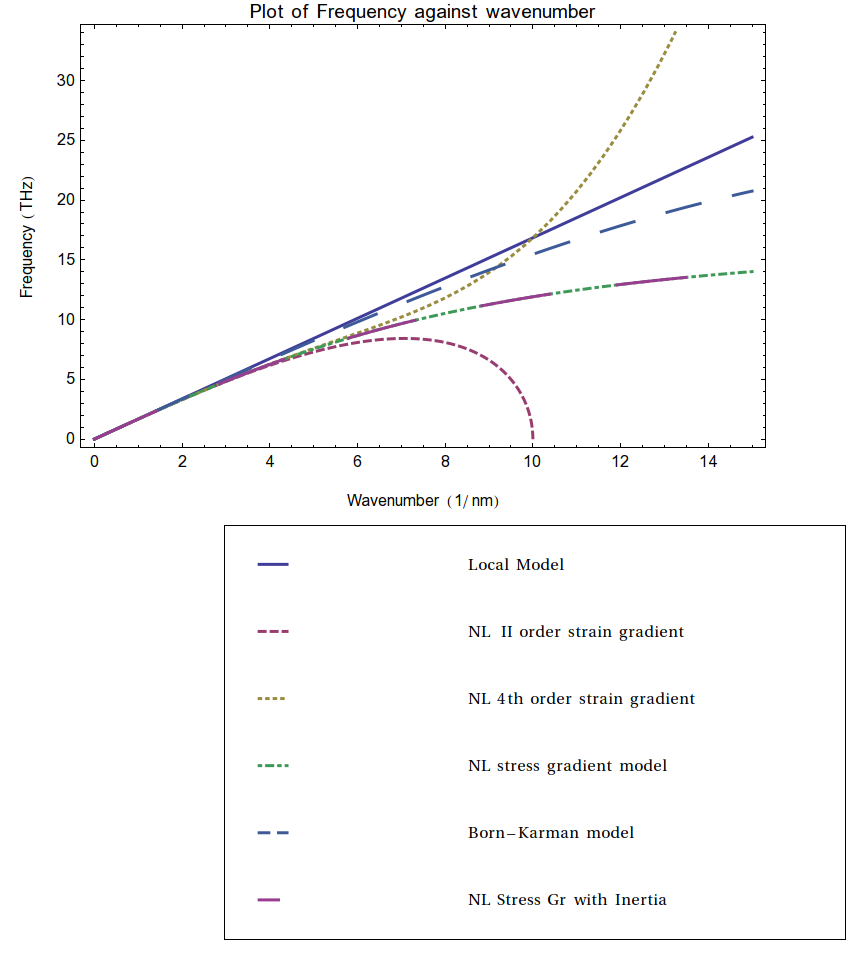
\includegraphics[scale=0.5]{terahertz_freq}
\caption{A Comparison of the wavenumber dispersion with wave frequency in a
nanorod obtained from classical/local and nonlocal theories suggested in literature
with the present result, to show the effect of lateral inertia.}
\label{terahertz_freqresp}
\end{figure}

The spectrum curves for nanorod obtained from both second
and fourth order strain gradient models are also shown in Fig. \ref{terahertz_freqresp}, for
comparison. As said, the spectrum relations obtained from the
classical continuum model shows that the waves in nanorod are
non-dispersive. But both the strain gradient models shows that the
waves in nanorod are dispersive in nature. It can also be seen that
the fourth order strain gradient model give improved approxima-
tion over the second order strain gradient model, as compared to
the classical continuum model (such observations are also made
in \cite{narendar2010ultrasonic}). The results are compared with the Born-K\'arm\'an model, as well as the nonlocal stress gradient model. This result shows an improved approximation over the second
order strain gradient model (see Fig. \ref{terahertz_freqresp}).It can be concluded that, the
instability of the second order strain gradient model can be
overcome by considering the inertia gradients.
The cut-off value for the wave number, i.e., the
wave number for which the angular frequency is zero, dominates
the static response of the second order strain gradient model. This cut-off emerges at $k=1/\sqrt{\alpha}$ (see Fig. \ref{terahertz_freqresp}). While for the fourth-
gradient model it only concerns the higher wave numbers, see
Fig. \ref{terahertz_freqresp}. However, in the response of the fourth order strain gradient model the effect of these high frequency waves are of minor
importance. Due to the nonuniqueness and instability of the second
order strain gradient model will give quite different wave behavior
compare to the fourth order strain gradient model. The unstable
second order strain gradient model can made stable by considering
the inertia gradients in the formulation.

The effect of the scaling parameter on the wave dispersion
relation in nanorod is shown in Fig. \ref{varyalpha}. As the nonlocal scaling
parameter $(\alpha = e_0 a)$ increases, the frequency of the wave will
decrease with an increase in the wavenumber. Here $\alpha$ values are
assumed from 0.0 to 1.0 nm. As $\alpha$ tends to larger value, the wave
frequency becomes very smaller at higher values of wavenumber as
shown in Fig. \ref{varyalpha}. It can be seen that, while dealing with the nonlocal
elasticity theory including the effect of lateral inertia, on should not
neglect the scaling parameter. So, the scaling parameter plays an
important role while dealing with the dynamics of nanostructures.

\begin{figure}
\centering
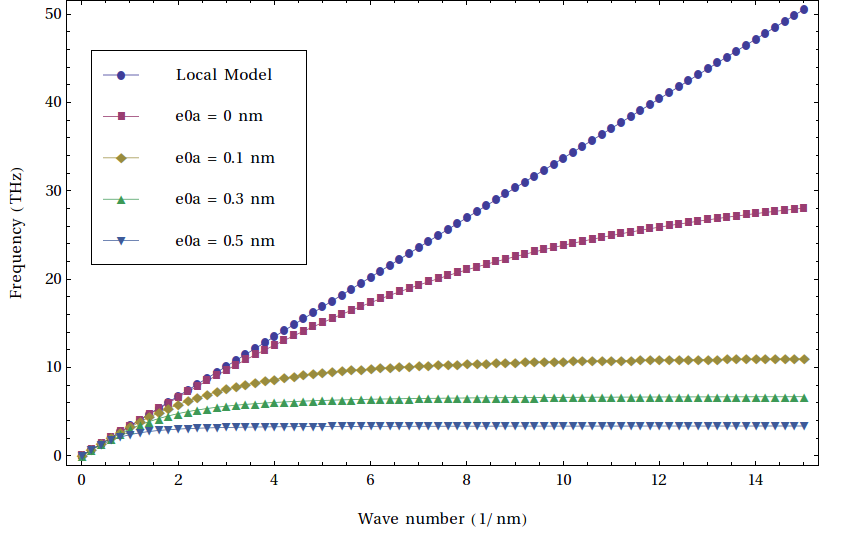
\includegraphics[scale=0.5]{tera_alphavary.png}
\caption{Wavenumber dispersion (including the effect of lateral inertia) with wave
frequency in a nanorod for various values of the nonlocal scaling parameter $\alpha$}
\label{varyalpha}
\end{figure}

The effect of radius of nanorod, on the wave dispersion relation
based on the present formulation is shown in Fig. \ref{varyradius}. For the present
analysis, we considered three different radii of nanorods i.e., 1.0,
2.0 and 5.0 nm. For comparison, the results obtained from local/
classical elasticity are also shown in the figure. As the radius of the
nanorod increases, the wave frequency becomes almost constant for
wavenumbers larger than 5.0 $\text{nm}^{-1}$. The effect of the lateral inertia
shows that, as the radius of the nanorod increases, the wavenumber
decreases and will not become constant irrespective of the wavenumber. The instability of the second order strain gradient
model can be overcome by considering the inertia gradients.

\begin{figure}
\centering
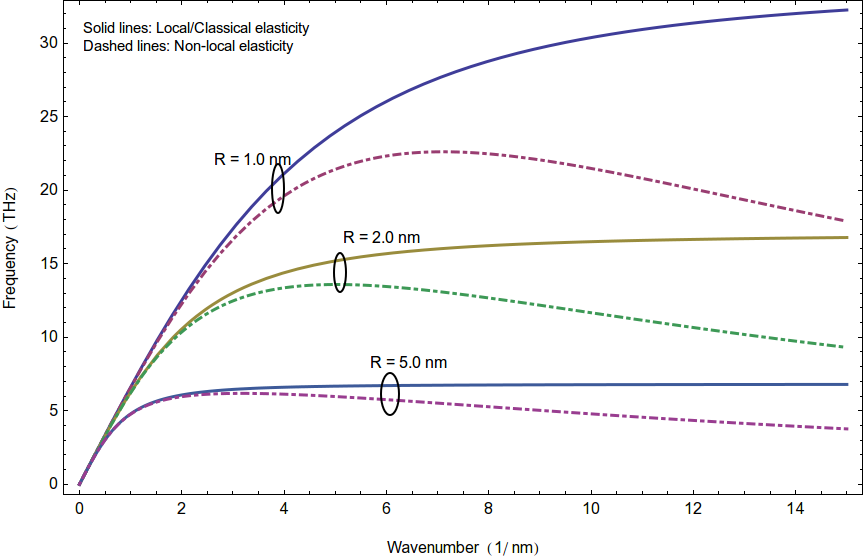
\includegraphics[scale=0.5]{varyradius.png}
\caption{Wavenumber dispersion (including the effect of lateral inertia) with wave
frequency in a nanorod obtained from both the local and nonlocal formulations for
different radii of nanorods.}
\label{varyradius}
\end{figure}

We have also analysed the behaviour of phase and group velocities using the models studied. This is illustrated in Fig. \ref{phasevel} and Fig. \ref{groupvel}. These plots also reinforce the observation that the strain gradient model (especially the second order strain gradient model) is not a stable model. Including lateral inertia in the stress gradient model indicates an improved response.

\begin{figure}
\centering
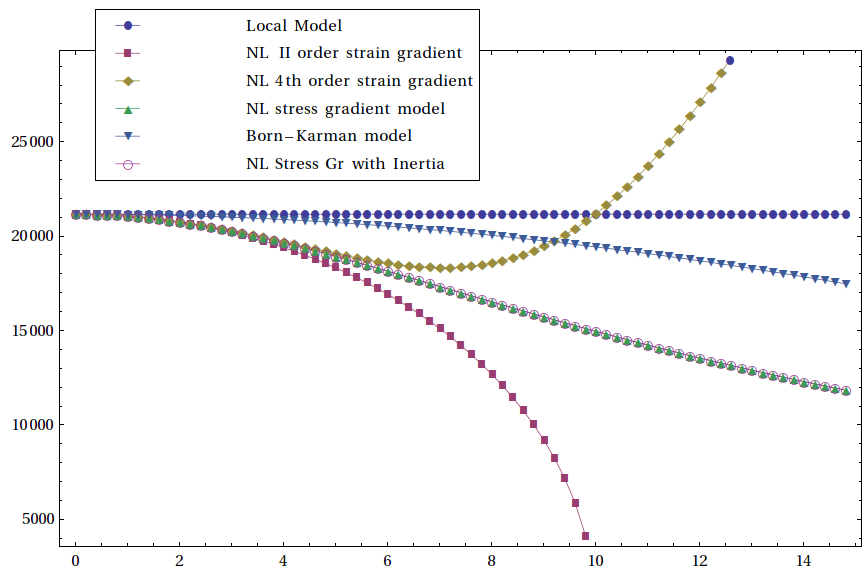
\includegraphics[scale=0.5]{phasevel.png}
\caption{Behaviour of phase velocity with varying wavenumber}
\label{phasevel}
\end{figure}

\begin{figure}
\centering
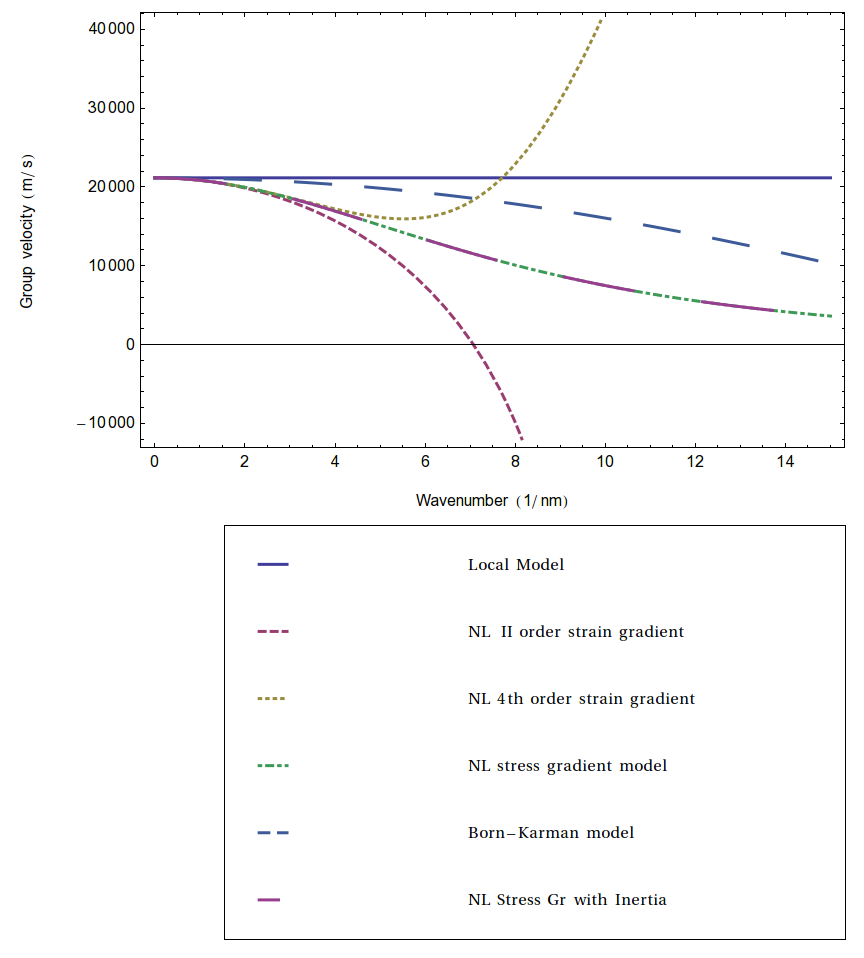
\includegraphics[scale=0.5]{groupvel.png}
\caption{Behaviour of group velocity with varying wavenumber}
\label{groupvel}
\end{figure}

It can be concluded that the wave dispersion characteristics in a
nanorod is drastically different for local and nonlocal models.
Where local model predicts that the wave will propagate at all
frequencies, but the nonlocal model shows that the wave will
propagate up to certain frequencies only depending on the nonlocal
scaling parameter. It has also been shown that, the unstable second
order strain gradient model can be replaced by considering the
inertia gradient terms in the formulations. 

\section{Axial wave propagation in coupled nanorod system with nonlocal small scale effects}

\chapter{Conclusion}
\input{chapters/conclusion.tex}
\bibliographystyle{unsrt}
\bibliography{refs}
\end{document}
